\chapter{Практическая реализация}
В этой главе описана реализация программ, которые моделируют и визуализируют некоторые из процессов, описанных ранее. В частности, разработаны программа моделирования квантовой части протокола релятивистского распределения ключей и программа моделирования процесса исправления ошибок протоколом Cascade.

\section{Используемые технологии и архитектура}
Обе программы написаны на языке C\# с использованием технологии Windows~Presentation~Framework (в дальнейшем WPF).
Язык C\# был выбран в частности из-за имеющихся в WPF встроенных богатых возможностей по анимации контента, что является весомым аргументов для программ визуализации.

\subsection{Описание выбранной архитектуры}
По рекомендации Microsoft, для программ, написанных на WPF, применялась архитектура MVVM (Model~--~View~--~ViewModel), ключевой особенностью которой является так называемая <<привязка данных>>, обеспечивающая изменение визуального состояния программы при изменении её внутреннего представления.

Шаблон MVVM состоит из трех частей:
\begin{itemize}
  \item Модель. Представляет собой фундаментальные данные и бизнес-логику, работающую с ними.
  \item Представление. Реализует пользовательский интерфейс и подписывается на события изменения Модели Представления. Когда изменяется какое-либо свойство Модели, она оповещает об этом всех подписчиков, Представление же запрашивает обновленное свойство из Модели Представления. В обратную сторону, действия пользователя над графическим интерфейсом приводят к вызову команд, определенных в МоделиПредставления, в результате выполнения которых может измениться состояние одной или нескольких Моделей.
  \item Модель Представления. Содержит в себе данные из Модели, подлежащие привязке, а также команды, которыми может пользоваться представление для влияния на Модель.
\end{itemize}

Таким образом происходит разделение бизнес-логики и логики отображения. Модель не знает ничего о том, кто и каким образом будет её использовать. Представление не знает ничего о том, откуда и как взялись данные, которые нужно отобразить, но знает о Модели Представления, чьи данные и команды следует использовать. Модель Представления имеет в себе ссылки на используемые Модели, но не знает, каким Представлением будет отображаться, поэтому предоставляет как свой интерфейс только обертки над данными модели и команды, обновляющие Модели. Более подробно шаблон будет рассмотрен ниже на конкретных примерах.

\subsection{Обзор используемых технологий визуализации}
Анимация~--- это иллюзия, которая создается последовательностью быстро сменяющихся изображений, каждое из которых немного отличается от предыдущего. Мозг получает группу изображений как цельную изменяющуюся сцену. В фильмах эта иллюзия создается с использованием камер, которые записывает множество кадров в секунду. Когда эти кадры воспроизводятся проектором, аудитория видит двигающуюся картинку.

Анимация на компьютере представляет собой примерно то же самое. Для примера, программа, в которой нарисованный прямоугольник плавно исчезает, может работать следующим образом:
\begin{enumerate}
  \item Программа создает таймер.
  \item Программа проверяет таймер через выставленные промежутки времени и смотрит, сколько прошло времени.
  \item Каждый раз, когда происходит проверка таймера, программа вычисляет текущее значение свойства прозрачности прямоугольника, основываясь на информации и прошедшем времени.
  \item После этого программа обновляет свойства прямоугольника их новыми значениями и перерисовывает его.
\end{enumerate}

До появления WPF разработчики были вынуждены создавать и поддерживать собственные системы тайминга или использовать чужие библиотеки. WPF включает в себя эффективную систему управления временем, которой можно пользоваться из управляемого кода и расширенного языка разметки приложения (XAML), и которая глубоко интегрирована в фреймворк WPF. Анимации WPF позволяют легко анимировать элементы управления и другие графические объекты.

WPF эффективно реализует в себе систему времени и перерисовки экрана. Он предоставляет специальные классы управления временем, чтобы разработчик мог сфокусироваться на том, какие эффекты он хочет создать, а не на механизме достижения этих эффектов.

Основной концепт анимаций в WPF~--- объекты анимируются путем применения анимации к конкретным свойствам этого объекта. К примеру, чтобы изменить плавно размер объекта, нужно применить анимацию к свойствам \mintinline{csharp}{Width} и \mintinline{csharp}{Height}. Чтобы заставить объект плавно исчезнуть, нужно анимировать свойство \mintinline{csharp}{Opacity}. Примеры задания анимации в XAML и в управляемом коде показаны в листингах \ref{lst:animations_in_xaml} и \ref{lst:animations_in_code} соответственно.

\begin{listing}[H]
\begin{xmlcode}
<Window x:Class="WpfApplication1.MainWindow"
        xmlns="http://schemas.microsoft.com/winfx/2006/xaml/presentation"
        xmlns:x="http://schemas.microsoft.com/winfx/2006/xaml"
        Title="MainWindow" Height="350" Width="525">
    <Grid>
        <StackPanel Margin="10">
            <Rectangle
                Name="MyRectangle"
                Width="100" 
                Height="100"
                Fill="Blue">
                <Rectangle.Triggers>
                    <!-- Animates the rectangle's opacity. -->
                    <EventTrigger RoutedEvent="Rectangle.Loaded">
                        <BeginStoryboard>
                            <Storyboard>
                                <DoubleAnimation
                                    Storyboard.TargetName="MyRectangle" 
                                    Storyboard.TargetProperty="Opacity"
                                    From="1.0" To="0.0" Duration="0:0:5" 
                                    AutoReverse="True" RepeatBehavior="Forever" />
                            </Storyboard>
                        </BeginStoryboard>
                    </EventTrigger>
                </Rectangle.Triggers>
            </Rectangle>
        </StackPanel>
    </Grid>
</Window>
\end{xmlcode}
\caption{Пример задания анимации в XAML.}
\label{lst:animations_in_xaml}
\end{listing}

\begin{listing}[H]
\begin{csharpcode}
namespace WpfApplication1
{
    public partial class MainWindow : Window
    {
        private Storyboard myStoryboard;

        public MainWindow()
        {
            InitializeComponent();

            StackPanel myPanel = new StackPanel();
            myPanel.Margin = new Thickness(10);

            Rectangle myRectangle = new Rectangle();
            myRectangle.Name = "myRectangle";
            this.RegisterName(myRectangle.Name, myRectangle);
            myRectangle.Width = 100;
            myRectangle.Height = 100;
            myRectangle.Fill = Brushes.Blue;

            DoubleAnimation myDoubleAnimation = new DoubleAnimation();
            myDoubleAnimation.From = 1.0;
            myDoubleAnimation.To = 0.0;
            myDoubleAnimation.Duration = new Duration(TimeSpan.FromSeconds(5));
            myDoubleAnimation.AutoReverse = true;
            myDoubleAnimation.RepeatBehavior = RepeatBehavior.Forever;

            myStoryboard = new Storyboard();
            myStoryboard.Children.Add(myDoubleAnimation);
            Storyboard.SetTargetName(myDoubleAnimation, myRectangle.Name);
            Storyboard.SetTargetProperty(myDoubleAnimation, new PropertyPath(Rectangle.OpacityProperty));

            // Use the Loaded event to start the Storyboard.
            myRectangle.Loaded += new RoutedEventHandler(myRectangleLoaded);
            myPanel.Children.Add(myRectangle);
            this.Content = myPanel;
        }

        private void myRectangleLoaded(object sender, RoutedEventArgs e)
        {
            myStoryboard.Begin(this);
        }
    }
}
\end{csharpcode}
\caption{Пример задания и запуска анимации в управляемом коде.}
\label{lst:animations_in_code}
\end{listing}

\section{Визуализация квантовой части релятивистского протокола распределения ключей}
Программа, визуализирующая процесс квантовой части протокола, была названа Requc (от Relativistic Quantum Cryptography) и в дальнейшем при необходимости будет использоваться именно это название.
Исходя из схемы протокола, в программе имеется две основных модели - модель квантового состояния и модель единичной посылки. 

Диаграмма классов представлена на рисунке \ref{fig:requc_models}
\begin{figure}[h]
  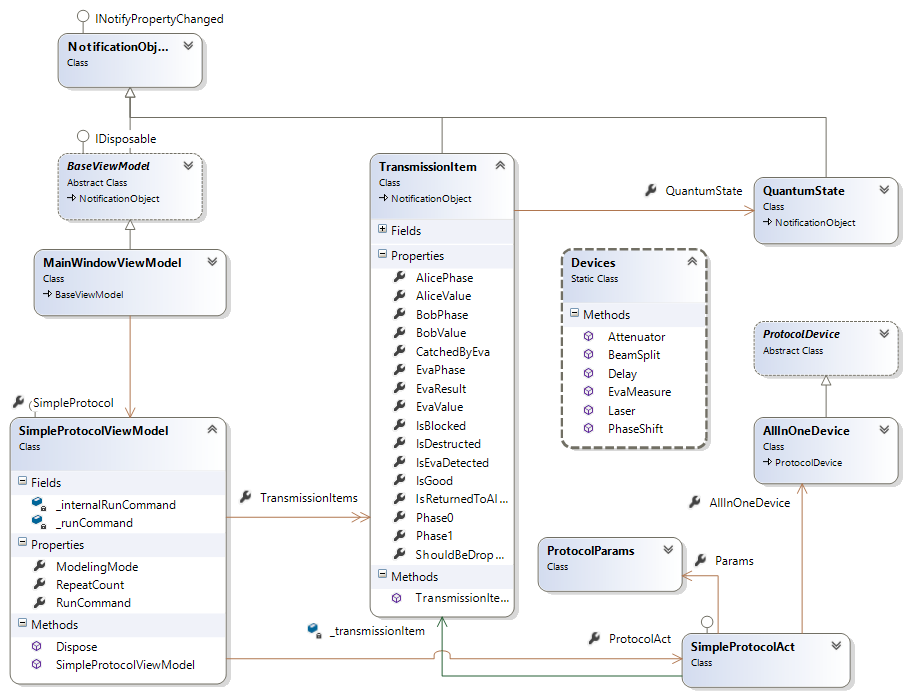
\includegraphics[width=0.9\linewidth]{chapter3/requc_models}
  \caption{Диаграмма классов программы Requc.}
  \label{fig:requc_models}
\end{figure}

Согласно описанному выше шаблону MVVM, все классы, имена которых оканчиваются на \textit{ViewModel}, являются Моделями Представлениями. 
В силу относительной визуальной простоты программы (нет сложной логики интерфейса, множества экранов и т.п.), по факту на протяжении всего жизненного цикла программы используется лишь одна модель представления~--- \mintinline{csharp}|SimpleProtocolViewModel|. Эта модель представления содержит ссылку на коллекцию объектов Модели \mintinline{csharp}|TransmissionItem|, представляющей собой объект посылки в протоколе, и ссылку на экземпляр Модели \mintinline{csharp}|SimpleProtocolAct|, который содержит метод (на схеме не указан) запуска очередной итерации протокола по описанной в пункте \ref{sec:common_description} схеме.

Главный экран программы показан на рисунке \ref{fig:requc_start_state}. В верхней части экрана по центру изображен оптический тракт между Алисой и Бобом с подслушивателем Евой в середине. В нижней части по центру изображена пространственно-временная плоскость. Слева от нее таблица с результатами каждого прохода. Справа вверху управляющие графические элементы, задающие режим моделирования, число повторений и запуск визуализации.
\begin{figure}[h]
  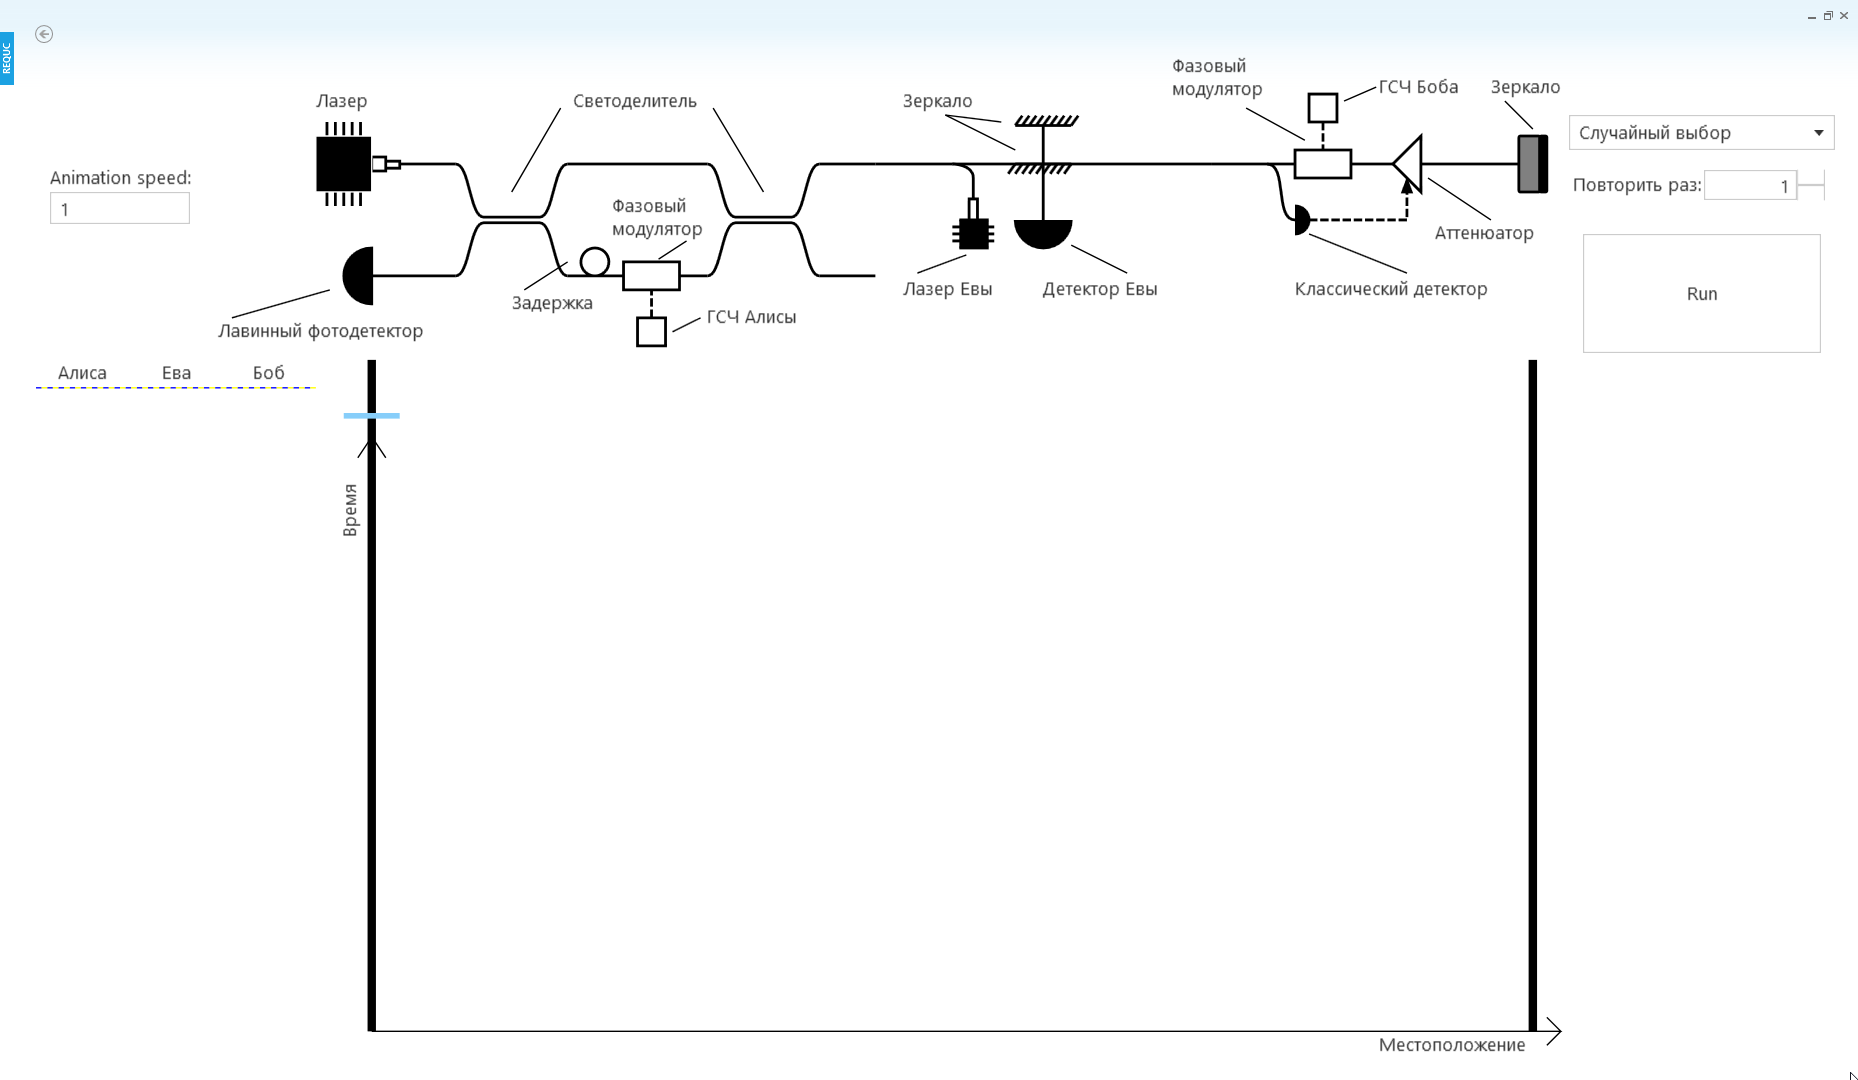
\includegraphics[width=0.9\linewidth]{chapter3/requc_start_state}
  \caption{Начальное состояние программы Requc.}
  \label{fig:requc_start_state}
\end{figure}

Данный экран отрисовывается Представлением \mintinline{csharp}|SimpleProtocolView|. Иерархия Представлений изображена на рисунке \ref{fig:requc_views}. Так как Представления не производят никаких действий над данными, а только отображают их, то жесткими связями, которые можно было бы изобразить на диаграмме классов, они не обладают, так как в принципе не содержат ссылок на экземпляры других Представлений или Модели представлений. Связывание данных происходит во время исполнения программы, и всю заботу об этом на себя берет WPF.
\begin{figure}[h]
  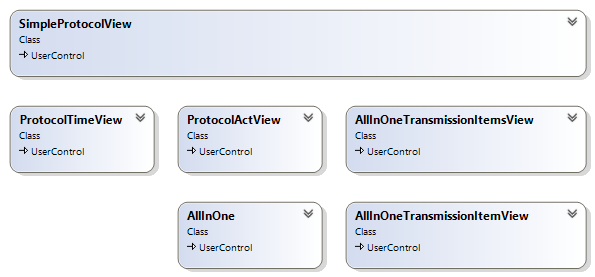
\includegraphics[width=0.9\linewidth]{chapter3/requc_views}
  \caption{Иерархия Представлений программы Requc.}
  \label{fig:requc_views}
\end{figure}




\section{Визуализация протокола исправления ошибок Cascade}